\documentclass[conference]{IEEEtran}
\IEEEoverridecommandlockouts
% The preceding line is only needed to identify funding in the first footnote. If that is unneeded, please comment it out.
\usepackage{cite}
\usepackage{amsmath,amssymb,amsfonts}
\usepackage{algorithmic}
\usepackage{graphicx}
\usepackage{textcomp}
\usepackage{xcolor}
\usepackage{listings}
\def\BibTeX{{\rm B\kern-.05em{\sc i\kern-.025em b}\kern-.08em
    T\kern-.1667em\lower.7ex\hbox{E}\kern-.125emX}}


\lstset{captionpos=b, numberbychapter=false,caption=\lstname,frame=none, numbers=left, stepnumber=1, numbersep=2pt, xleftmargin=2pt, framexleftmargin=2pt, numberstyle=\tiny, tabsize=3, columns=fixed, basicstyle={\fontfamily{pcr}\selectfont\footnotesize}, keywordstyle=\bfseries, commentstyle={\color[gray]{0.33}\itshape}, stringstyle=\color[gray]{0.25}, breaklines, breakatwhitespace, breakautoindent}
\lstloadlanguages{[ANSI]C, C++, [gnu]make, gnuplot, Matlab}

\begin{document}

\bibliographystyle{IEEEtran}

\title{Microservices: Use of REST and gRPC over SOAP}

\author{\IEEEauthorblockN{Marcel Gredler}
\IEEEauthorblockA{\textit{Computer Science} \\
\textit{FH Technikum Wien}\\
Vienna, Austria \\
se19m025@technikum-wien.at}
\and
\IEEEauthorblockN{Florencia Cavallin}
\IEEEauthorblockA{\textit{@Florencia (department)} \\
\textit{@Florencia (uni)}\\
@Florencia (city), Argentina \\
fcavallin@itba.edu.ar}
}

\maketitle

\begin{abstract}

Since the induction of Web Services into modern applications, their usage has grown. Together with them the general public was first introduced to the use of protocols like the Simple Object Access Protocol (SOAP) and Representational State Transfer (REST).

In more recent years a new trend started emerging in the development of applications, in which the application is split into a set of small services that use a communication protocol to interact with another. This trend is known as the Microservice Architecture and it favors the use of REST, a Message Bus or other stateless communication protocols over SOAP.

This paper gives an overview of the Microservice Architecture, explains why the use of REST is favored over SOAP and how the new gRPC Remote Procedure Calls (gRPC) framework may support them.

\end{abstract}

\begin{IEEEkeywords}
services, rest, grpc, microservices
\end{IEEEkeywords}

\section{Introduction}

Nowadays their exist many different paradigms and architectures that can be used to create applications. One of these architectural styles is the Service Oriented Architecture (SOA), in which the functionality is split between multiple services that may be run locally or be distributed around the network.

One methodology that heavily uses this paradigm and that is in widespread use, are web services \cite{halili2018web}. Within the use of web services applications can benefit by reusing the functionality of already existing other services. Because of this it is possible to reduce the need of rewriting existing functionality into every application. Another benefit is the possibility of sharing information between all such web services. To achieve all these benefits, web services traditionally employ the Simple Object Access Protocol (SOAP) or Representation State Transfer (REST) protocols \cite{halili2018web}.

Another methodology that became widespread between 2010 and 2020 are microservices. Where web services focused on offering a full service to another application or user, microservices are built around the offering and using of capabilities \cite{karmel2016nist}. Each capability is thereby built and offered as its own service and all communication is performed through an Application Programming Interface (API). A set of microservices can therefore build an application or be used to provide capabilities to other applications.

Since microservices are using lightweight protocols \cite{karmel2016nist} to communicate with each other, a protocol like REST is preferred over SOAP. One of the biggest advantages of REST over SOAP is the smaller payload, as SOAP may require the services to exchange ten times more bytes between each other in comparison to REST \cite{halili2018web}. Since microservices are built around capabilities and interaction between each other, a smaller payload allows for better use of the available bandwidth.
Additionally, changing the provisioning in SOAP may require changes on the clients, whereas REST does not \cite{halili2018web}. This is another important advantage, as microservices are generally designed to be independently deployable \cite{karmel2016nist}, which would be broken, if the deployment of one service requires the deployment of another.

With the from 2015 slowly emerging HTTP/2 standard \cite{rfc7540} another communication framework has been developed: gRPC Remote Procedure Calls (gRPC) \cite{GRPCAuthors2020}. While previously microservices only used REST, this new framework allows for the use of both gRPC and REST to interact with another. The gRPC framework thereby offers the ability to build so called gRPC REST Gateways \cite{grpcrest}. These gateways are proxies for that expose the gRPC capability through REST. This means that other services are able to use them with gRPC - if they so support this too - or use the REST API. The latter is especially useful in networks where HTTP/2 traffic is not yet fully supported, if for example used loadbalancer only support HTTP/1.1 yet.

This paper gives an introduction of the mentioned protocols SOAP, REST and gRPC. Furthermore it explains what microservices are and how the compare to a classical service oriented architecture. Lastly, the document explains the benefit of using HTTP/2 and gRPC in conjunction with a microservice architecture.

To achieve this goal, the paper is structured as follows: Sections \ref{sec:soap} to \ref{sec:grpc} cover the explanation about SOAP, REST and gRCP respectively. Section \ref{sec:micros} is about microservices and their comparison to the service oriented architecture. This is followed by section \ref{sec:comp} which contains the benefit of using HTTP/2 and gRPC and REST. And lastly, the document finished by providing a conclusion about the use of gRPC and REST in microservices.

\section{SOAP}
\label{sec:soap}

\section{REST}

\section{HTTP/2}

The state of the web report of the HTTP archive \cite{httpArchive} suggests that between December 2010 and 2020, the amount of kilobytes (KB) required to load a web page increased by about 318 percent. In other words, in 2010 a page consisted of a median 487.9 KB, whereas in 2020 a web page consists of 2042.3 KB. Such an increase in size is a challenge for both the network we use and the protocols our communication is built upon.

HTTP/1.1 tries to solve the problem of increased page sizes by allowing request pipeline and through the use of multiple parallel open connections. While this was a viable approach for many years, an IETF working group published the newer HTTP/2 specification RFC 7540 \cite{rfc7540} in 2015, with an update regarding TLS 1.3 having been published in RFC 8740 \cite{rfc8740}. This new protocol version promises to solve the problems of HTTP/1.1 that prevent it from being more efficient.

Protocol version HTTP/2 moves away from sending text over the web and instead replaces it with binary data. RFC 7540 \cite{rfc7540} and the IETF HTTP working group \cite{httpwgHTTP2} explain this decision through the argument that binary data is more efficient to parse, as it less error prone and does not require to keep traffic of special characters in the data.

Furthermore HTTP/2 reworks the way semantic information is send through the web (see RFC 7540 \cite{rfc7540} for details) with the goal of allowing multiple requests to be sent through the same connection. Based on the documents \cite{rfc7540} \cite{httpwgHTTP2} this decisions has been to make the HTTP/2 protocol more in line with how TCP connections work. For traffic to flow through an TCP connection, a handshake has to be done first between the two participants. In HTTP/1.1 this meant that for each parallel request a newly opened connection had to go through this very handshake again, instead of being able to use the handshake from the first request, overall increasing the overhead a user had to perform to download the content of a page. HTTP/2 on the other hand only opens one TCP connection minimizing this overhead. Additionally, the header of the HTTP/2 protocol itself are compressed while being send through the network, further reducing the size of each message.

Lastly, HTTP/2 introduces a new feature called server push \cite{rfc7540}. With this feature it is possible for a server to push additional information to the clients, based on their previous requests, without having to wait for them to open a request for this data themselves. Though introducing the ability to send "false-positive" data (i.e. data that is not used by the user in the end), this new feature allows the server to provide the user with "future" information without delay (from user perspective), which helps in providing a better user experience.

\begin{table}[!htbp]
	\centering
	\caption{HTTP/1.1 VS HTTP/2}
	\label{http2comparison}
	\begin{tabular}{| p{0.4\linewidth} | p{0.4\linewidth}|}\hline
		HTTP/1.1 & HTTP/2 \\\hline
		text-based protocol & binary protocol \\\hline
		one request per TCP connection & multiple requests per TCP connection \\\hline
		no header compression & header compression \\\hline
		only client may request data & client may request data and server may push additional data \\\hline
	\end{tabular}
\end{table}

To further highlight these core differences between how HTTP/1.1 and HTTP/2 treat their traffic, table \ref{http2comparison} provides a comparison of the two versions, reiterating the information provided by this section in a compact format.

The claims of performance improvement by use of HTTP/2 instead of HTTP/1 can be validated empirically. Corbel, Stephan and Omnes perform in their paper "HTTP/1.1 pipelining vs HTTP2 in-the-clear: Performance comparison" \cite{7745823} such an empirical study. They compare the time to download web pages by using the same infrastructure and server, with only the protocol version differing in the data-sets. As a result of their study they were able to identify that HTTP/2 truly does perform better than HTTP/1 for downloading content.

\section{gRPC}
\label{sec:grpc}

The gRPC Remote Procedure Calls (gRPC) framework \cite{GRPCAuthors2020} is a technology initially developed by Google and since having been become an open source framework maintained by the Cloud Native Computing Foundation (CNCF). It is a remote procedure call (RPC) framework that has been developed in modern times (2015 and onwards) and is backed by the HTTP/2 protocol. It has been created with the idea of a general purpose RPC infrastructure and microservice architecture in mind. This means that the created RPC framework was required to be language agnostic and allow for the fast and responsive intercommunication between a multitude of service instances. 

Above requirements to the RPC protocol are reflected by the following principles of the gRPC design specification \cite{grpcmotiviation}:

\begin{itemize}
	\item \textbf{Services not objects}: gRPC allows for the communication with services and is not an object oriented.
	\item \textbf{Messages not References}: Client and server exchange messages between them and do not have references to objects.
	\item \textbf{Interoperability \& Reach}: "The wire protocol must be capable of surviving traversal over common internet infrastructure." \cite{grpcmotiviation}
	\item \textbf{General Purpose}: The framework should be usable with most use-cases.
	\item \textbf{Performant}: The framework should not perform significantly worse when compared to a framework designed for a specific use-case.
	\item \textbf{Payload Agnostic}: gRPC needs to supports different message types (protcol buffers, JSON, XML, Thrift) and compression mechanisms.
	\item \textbf{Streaming}: The framework allows for server responses and clients requests to be send in a stream.
	\item \textbf{Blocking}: gRPC supports synchronous communication.
	\item \textbf{Non-Blocking}: gRPC supports asynchronous communication.
\end{itemize}

\begin{figure}
	\centering
	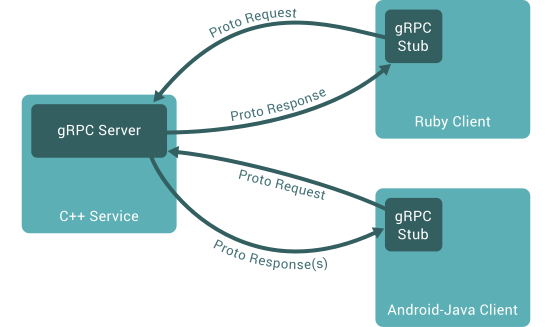
\includegraphics[width=0.8\linewidth]{grpc1.png}
	\caption{Abstract example of different clients using gRPC (Image downloaded from https://grpc.io/docs/what-is-grpc/introduction/ in January 2021)}
	\label{fig:grpcuse}
\end{figure}

As with other RPC frameworks, gRPC allows the client to perform operations as if they were run on the clients machine. For this the client needs to be aware of method definition and location of the remote server. To describe these methods gRPC uses protocol buffers \cite{protoBuffer} as the default interface description language (IDL), but it is possible to use other formats (like JSON) through the use of gRPC extensions. Protocol buffers themselves are a format developed by Google and used to serialize and deserialize structured data. Google describes this format as "think XML, but smaller, faster and simpler" \cite{protoBuffer}. 

A high-level abstraction of the gRCP intercommunication is shown in figure \ref{fig:grpcuse}. Within this image the gRPC server is written using C++ code. But because of the language agnostic of gRPC an android phone with a Java client is able to use communicate with this server, the same way a ruby client is able to communicate with the server.

\begin{lstlisting}[name={Small sample proto buffer specification (Full example available at https://grpc.io/blog/coreos/)},label={code:grpcproto}]  % Start your code-block

service EchoService {
	rpc Echo(EchoMessage) returns (EchoMessage) {
		option (google.api.http) = {
			post: "/v1/echo"
			body: "*"
		};
	}
}
\end{lstlisting}

\begin{figure}
	\centering
	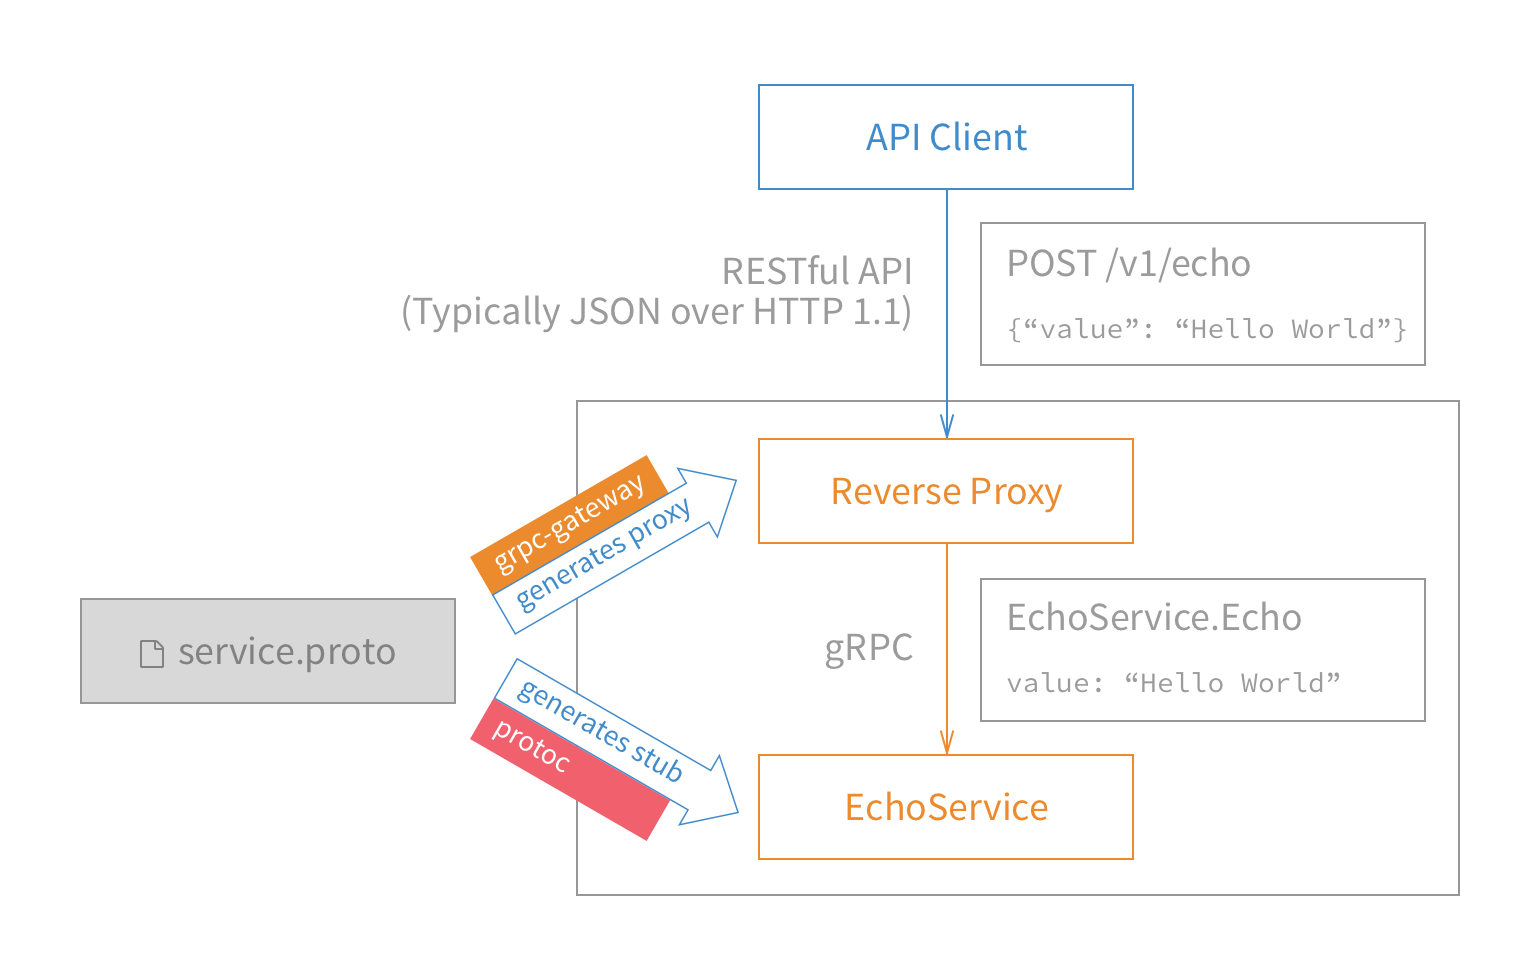
\includegraphics[width=0.8\linewidth]{grpc-rest-gateway.png}
	\caption{Example use of created rest-proxy to communicate with gRPC server (Image downloaded from https://grpc.io/blog/coreos/ in January 2021)}
	\label{fig:restProxy}
\end{figure}

Though gRPC has many advantages in its favor, the framework has the problem that it is requiring the HTTP/2 streaming functionality and the protocol HTTP/2 itself to work. As HTTP/2 is still relatively new, not all companies have their infrastructure supporting HTTP/2. As a backwards compatibility to HTTP/1.1 and for general automation support (i.e. no need to import and use stub code), gRPC IDL information can be enhanced with REST options, as shown in listing \ref{code:grpcproto} These changes will cause the compilation to create a rest-proxy in addition to the actual gRPC server. When a client now wants to communicate through REST, it may talk with the rest-proxy, which in turn will forward the requests through gRPC to the actual gRCP server. Figure \ref{fig:restProxy} illustrates this communication path and additionally highlights how the created services are based on the same IDL specification.

As previously mentioned, this makes it possible to have gRPC server and services running within an HTTP/1.1 infrastructure. By HTTP/1.1 infrastructure is hereby meant that not all network components within the infrastructure support the HTTP/2 protocol and have the connections fall back to HTTP/1.1 when trying to communicate through them. Such components could be router, loadbalancer or even the web-server.

\section{Microservices}
\label{sec:micros}

As the purpose of this paper is to identify the use of REST and gRPC over SOAP in microservice architectures, it is necessary to declare the definition that is used for the term microservice. The internet has multiple possible uses of the term microservice and they may vary on the blogs or scientific papers visited. For the purpose of this document, the definition of the national institute of standard and technology (NIST) is used:

"\emph{Microservices: A microservice is a basic element that results from the architectural decomposition of an application’s components into loosely coupled patterns consisting of self-contained services that communicate with each other using a standard communications protocol and a set of well-defined APIs, independent of any vendor, product or technology.}" - NIST \cite{karmel2016nist}

\begin{table}[!htbp]
	\centering
	\caption{Comparison of SOA and Microservices (Karmel, Anil
		Chandramouli, Ramaswamy
		Iorga, Michaela, 2016)}
	\label{micro:comparison}
	\begin{tabular}{| p{0.4\linewidth} | p{0.4\linewidth}|}\hline
		Service Oriented Architecture & Microservice \\\hline
	Self-contained, monolithic services & Small, decomposed, isolated and independently deployable services Communications\\\hline
		Communications between services occur through an enterprise service bus & Communications between services occur through lightweight, standard communications protocols and interfaces\\\hline
		Stateful and requires mapping of service dependencies when changes are introduced & Stateless and less fragile when changes are introduced\\\hline
		Longer start/stop times & Quick start/stop times\\\hline
		Built around services & Built around capabilities\\\hline
	\end{tabular}
\end{table}

Looking at this definition it can be seen that microservice architectures are based on service oriented architectures, but they drive the decomposition of applications even further. Document "Nist definition of microservices, application containers and system virtual machines" \cite{karmel2016nist} provides us with a comparison between a "standard" SOA and microservice architecture, see table \ref{micro:comparison}. Based on this comparison it can be seen that microservices decompose an application not just into services but into capabilities. These capability services are to be stateless and allow for independent, fast deployments. In section \ref{sec:comp} the paper focuses on how these differences between SOA and microservices have brought about the trend of using REST and gRPC instead of SOAP in microservice architectures.

\section{Comparison of Protocols}
\label{sec:comp}

\begin{table}[!htbp]
	\centering
	\caption{Comparison between SOAP and REST (Wagh \& Thool, 2015)}
	\label{fig:compSoapRest}
	\begin{tabular}{| p{0.4\linewidth} | p{0.4\linewidth}|}\hline
		SOAP & REST \\\hline
		Changing services in SOAP web provisioning often means a complicated code change on the client side. & Changing services in REST web provisioning not requires any change in client side code\\\hline
		SOAP has heavy payload as compared to REST & REST is definitely lightweight as it is meant for lightweight data transfer over a most commonly known interface, - the URI
		It\\\hline
		It requires binary attachment parsing. & It supports all data types directly.\\\hline
		%SOAP is not a wireless infrastructure friendly. & REST is a wireless infrastructure friendly\\\hline
		SOAP web services always return XML data. & While REST web services provide flexibility in regards to the type of data returned.\\\hline
		It consumes more bandwidth because a SOAP response could require more than 10 times as many bytes as compared to REST. & It consumes less bandwidth because it’s response is lightweight.\\\hline
		SOAP request uses POST and require a complex XML request to be created which makes response-caching difficult. & Restful APIs can be consumed using simple GET requests,
		intermediate proxy servers /
		reverse-proxies can cache their response very easily.\\\hline
		SOAP uses HTTP based APIs refer to APIs that are exposed as one or more HTTP URIs and typical responses are in XML / JSON. Response schemas are custom per object & REST on the other hand adds an element of using standrdized URIs, and also giving importance to the HTTP verb used (i.e. GET / POST / PUT etc)\\\hline
		Language, platform, and transport agnostic. & Language and platform agnostic\\\hline
		Designed to handle distributed computing environments. & Assumes a point-to-point communication model—not for distributed computing environment where message may go through one or more intermediaries\\\hline
		Harder to develop, requires tools. & Much simpler to develop web services than SOAP\\\hline
		False assumption: SOAP is more secure. SOAP use WS-Security. WS-Security was created because the SOAP specification was transport-independent and no assumptions could be made about the security available on the transport layer. & REST assumes that the transport will be HTTP (or HTTPS) and the security mechanisms that are built-in to the protocol will be available\\\hline
		%Is the prevailing standard for web services, and hence has better support from other standards (WSDL, WS) and tooling from vendors. & Lack of standards support for security, policy, reliable messaging, etc., so services that have more sophisticated requirements are harder to develop.\\\hline
	\end{tabular}
\end{table}

// use of table \ref{fig:compSoapRest} as basis for the three protocols

// use microservice definition and table \ref{micro:comparison} as basis for ms requirements

// I commented the rows that are (based on my opinion) not relevant for our comparison

I would say our arguments should be (as to why microservices use rest):
\begin{enumerate}
	\item support of data types
	\item payload size / bandwith
	\item deployment frequency: MS is deploy fast and often; the REST where changes are easier is therefore preferred
	\item point-to-point communication (based on MS definition)
	\item easier to develop REST than SOAP
\end{enumerate}

These 5 points are the main points based on what I can find in the tables and definitions. Additionaly, it nicely correlates to my personal experiences to why people prefer REST than SOAP (making me feel that my observation is valid; your opionion please :) )

-> afterwards I would make the observation how gRPC can help / support. For this I would just take the "REST" column of table \ref{fig:compSoapRest} and compare it with a "gRPC" column. And then make some observations based on that.

\section{Conclusion}

We split the heavens and conquer the earth!

\bibliography{IEEEabrv,literature}

\end{document}
